%----------------------------------------------------------------------
% MAIN PROGRAM OF THESIS
%----------------------------------------------------------------------

% Set the class of document by NYCU
% Availbale Class:
%   模式:[draft] | final (初稿 | 定稿)
%   用途:[print] | upload (輸出 | 上傳)
\documentclass[final, print]{Class/NYCUtran}

%----------------------------------------------------------------------
% 參數設定們
%----------------------------------------------------------------------

% 請去Config/config.tex填一些關於這本論文的參數
%----------------------------------------------------------------------
% CONFIGURATION
% 這邊就是一些等一下模板在生出像是封面這些東西的時候,會需要用到的參數
%----------------------------------------------------------------------

% 中英文論文題目
\zhTitle{中文論文題目}
\enTitle{English Thesis Title}

% 中英文關鍵字
%       依據學校規定,關鍵詞 5-7 個,應附於摘要內
\zhKeywords{關鍵字一、關鍵字二、關鍵字三、關鍵字四、關鍵字五}
\enKeywords{Keyword1, Keyword2, Keyword3, Keyword4, Keyword5}

% 研究生中英文姓名
%       依據學校提供的範例,英文姓名應寫「姓, 名」,例:Wang, Jing
\zhStudentName{中文研究生姓名}
\enStudentName{English Name}

% 指導教授中英文姓名
%       依據學校提供的範例,英文姓名應寫「姓, 名」,例:Wang, Jing
\zhAdvisorName{指導教授姓名}
\enAdvisorName{Advisor's English Name}

% 中英文學校名稱
\zhUnivName{國立陽明交通大學}
\enUnivName{National Yang Ming Chiao Tung University}

% 中英文學院名稱
\zhCollegeName{資訊學院}
\enCollegeName{College of Computer Science}

% 中英文研究所名稱
\zhInstName{資訊科學與工程研究所}
\enInstName{Institute of Computer Science and Engineering}

% 英文領域名稱
%       書名頁要用的
\enField{Network Engineering}

% 英文地點名稱
%       書名頁要用的
%       依據學校提供的範例,Taiwan, Republic of China
\enLocation{Taiwan, Republic of China}

% 論文日期
\zhDegreeYear{一一○}
\zhDegreeMonth{七}
\enDegreeYear{2021}
\enDegreeMonth{July}

% 論文浮水印
% 抱歉,窩沒做這個功能,因為窩沒有校徽可以放QQ
% 請去Config/fonts.tex填一下要用的字體
%-------------------------------------------------------------------------------
% 字體設定
% 拜託填一下要用的中文字型
%-------------------------------------------------------------------------------

% 中文字體
%       - 其實學校沒規定,內頁的字型要用啥,但是應該大部分都是用「標楷體」才對。
%           請填上系統的標楷體的名稱是是啥,請不要留空。如果留空的話,會直接編失敗喔。
%       - 窩知道的名稱只有底下二個
%           Windows:標楷體
%           Overleaf:cwTeXKai
%           其他系統:窩不知道
\zhFont{標楷體}

% 英文字體
%       - 其實學校沒規定,內頁的字型要用啥,但是應該大部分都是用「Times New Roman」才對。
%           請填上系統的對應的名稱是是啥,請不要留空。如果留空的話,會直接編失敗喔。
\enFont{Times New Roman}

% 等寬字體
%       - 其實學校沒規定,啥時要用等寬字,等寬字的字體要用啥。
%           這邊可以留空,因為TeX有預設的字體,最多會跳一些Warning出來啦。
\ttFont{}

%----------------------------------------------------------------------
% MAIN CONTENT
%----------------------------------------------------------------------

\begin{document}


% 以下註解的數字編號是參考自
% https://aa.nycu.edu.tw/reg/regulation/ 
%    底下的 博碩士學位論文格式規範(中、英文說明)
% 窩有留一份在Others裡面

% 1. 封面頁
\coverPage

% 2. 書名頁
\titlePage

% 3. 論文電子檔著作權授權書
%       - 這邊提供的是學校的公版文件
%           https://aa.nycu.edu.tw/reg/regulation/
%       - 口試完將修改完的論文上傳到
%           https://etd.lib.nctu.edu.tw/cgi-bin/gs32/tugsweb.cgi?o=dwebmge
%           就會拿到填好的各種授權書
%           這不是初稿應和上傳版本該出現這些東西才對
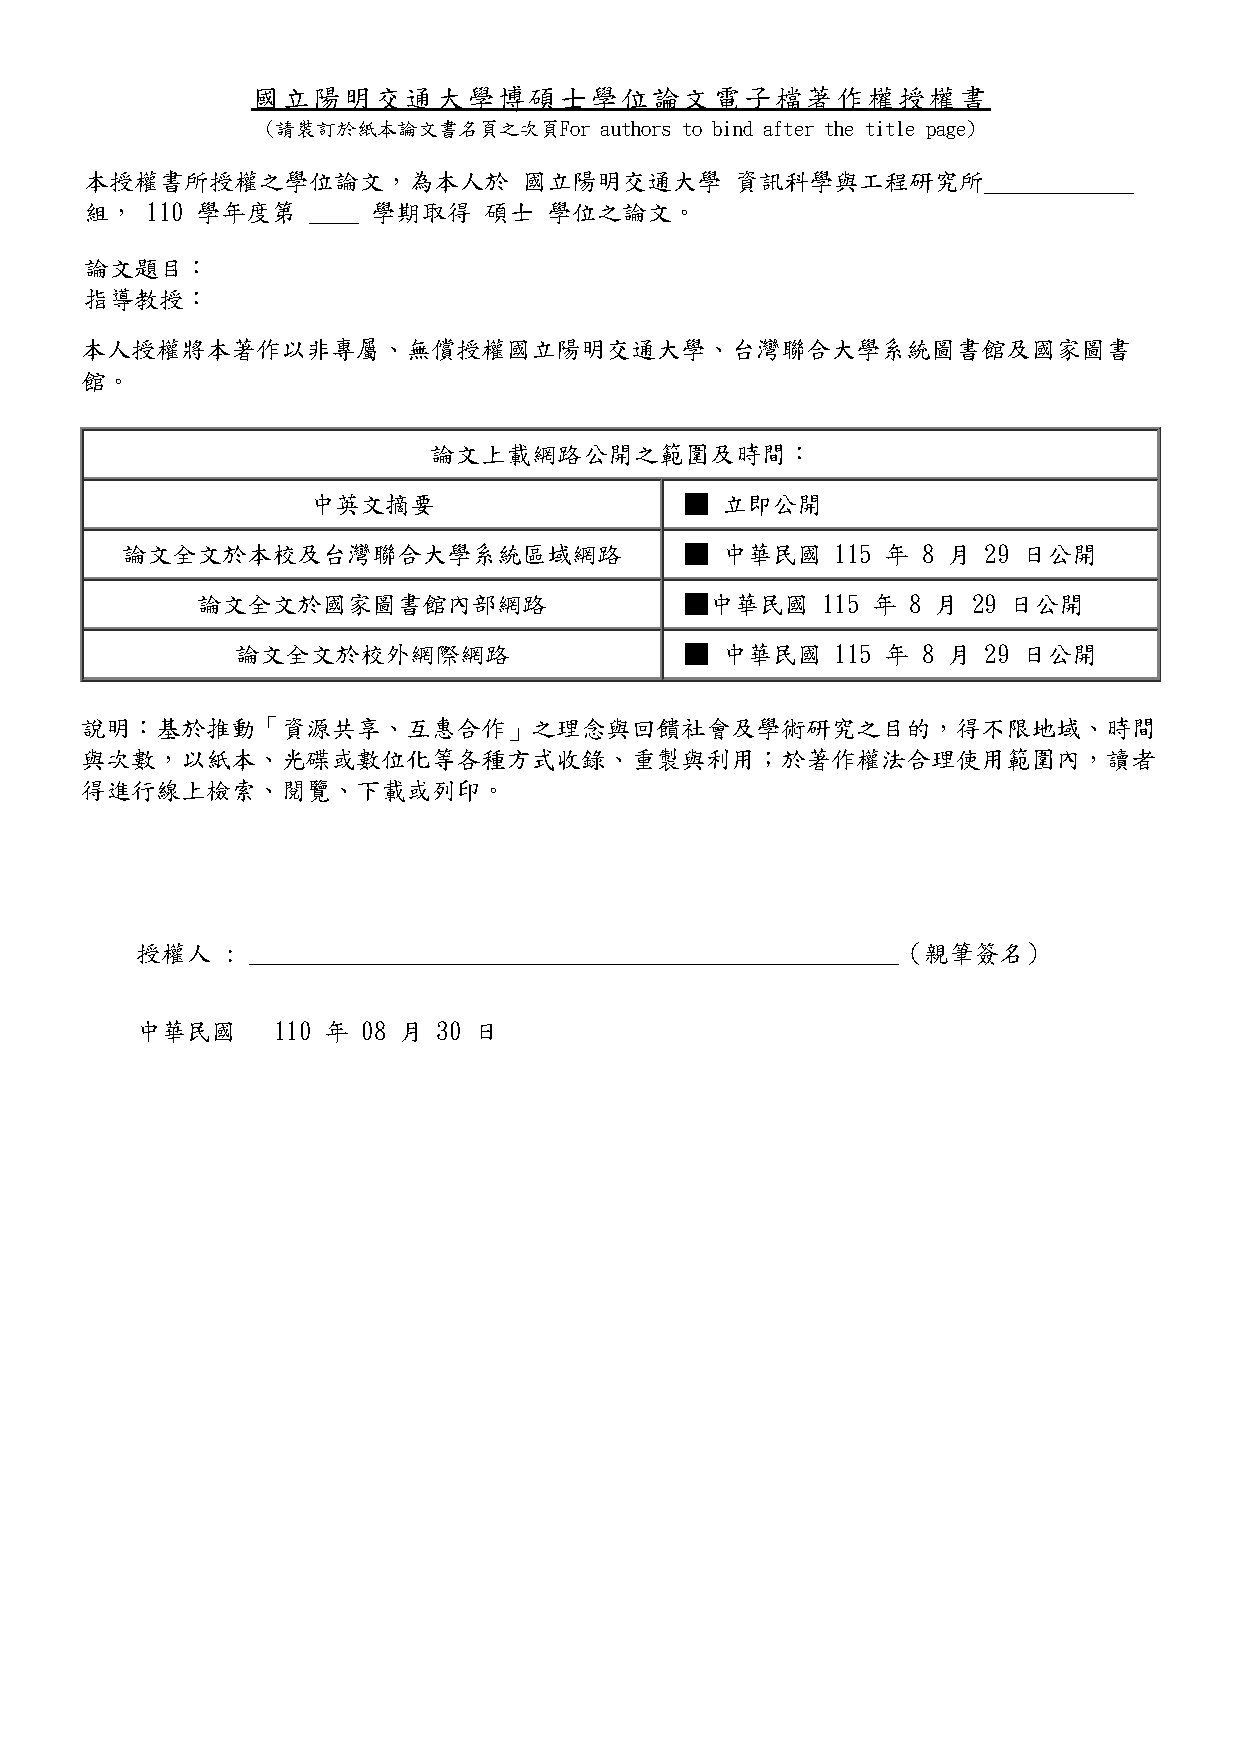
\includepdf[pages={1}]{1-Authorization/1-Authorization.pdf}
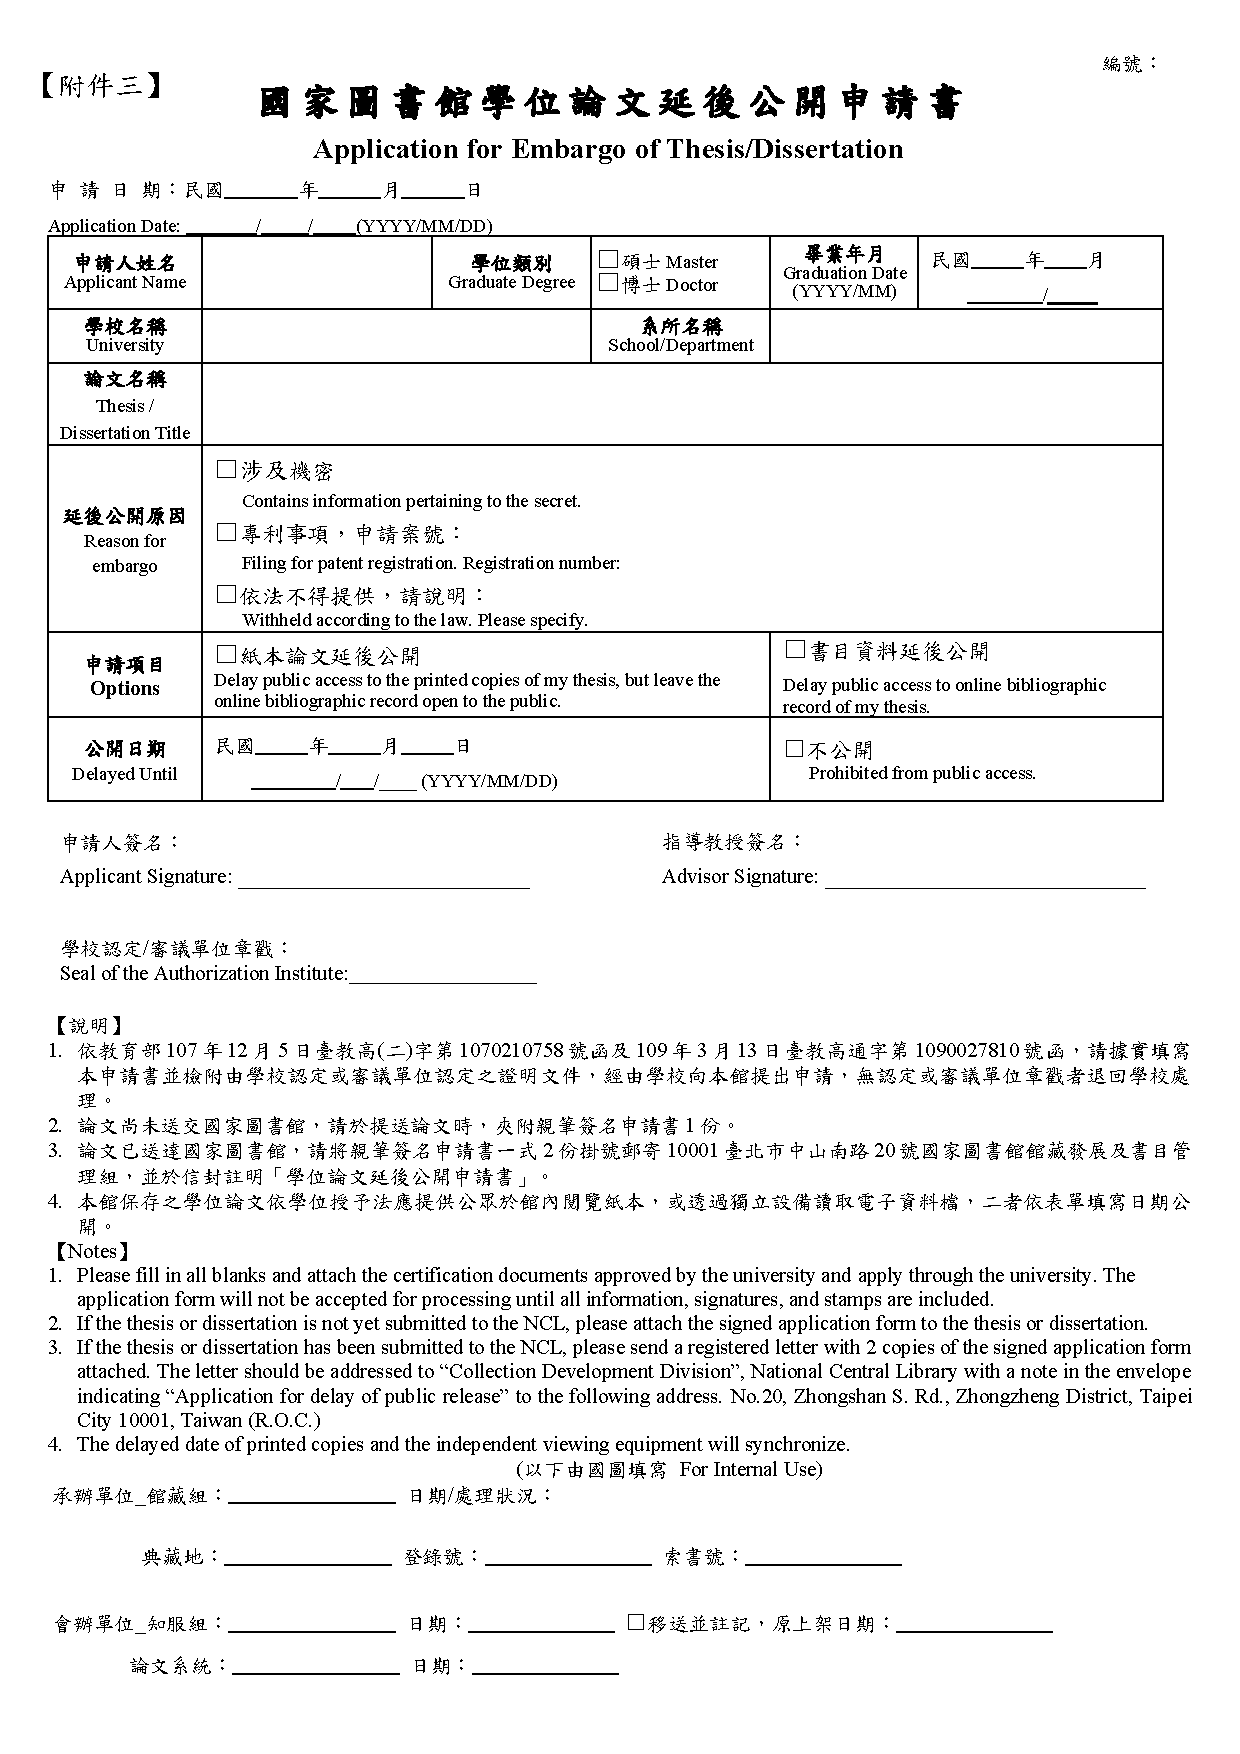
\includepdf[pages={1}]{1-Authorization/2-PostponePublication.pdf}

% 5. 論文審定同意書
%       - 這邊有附一個學校提供的公版
%           https://aa.nycu.edu.tw/reg/regulation/
%           但假如是資訊學院的同學,可以直接在申請口試完後從系統匯出已經填好資料的這張表
%       - 這一頁將不會出現在上傳版本中(學校的電子論文不需要這一張),只會出現在列印輸出版中
%           這個也是口試完才會有完整簽名的東西,所以初稿也不會出現這頁
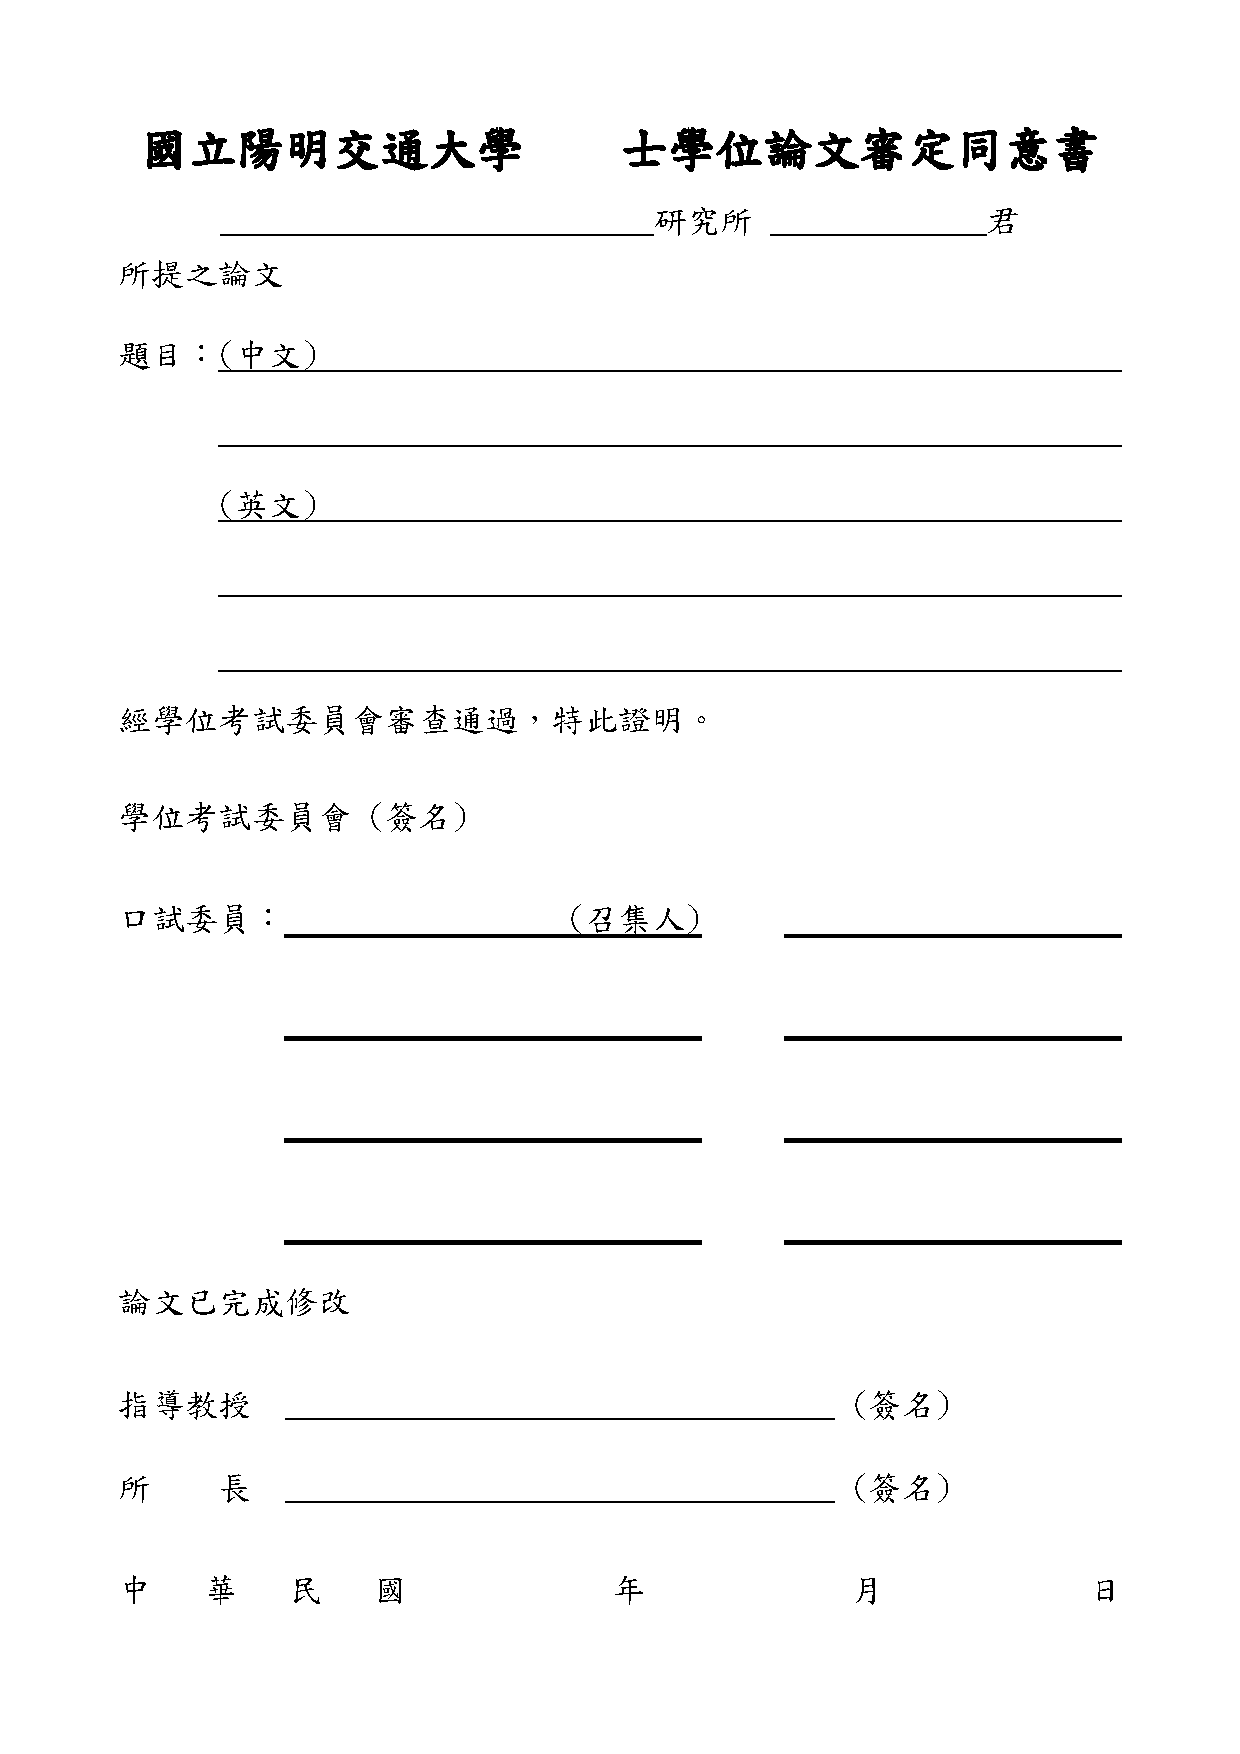
\includepdf[pages={1}]{2-Approval/1-Approval_zh.pdf}
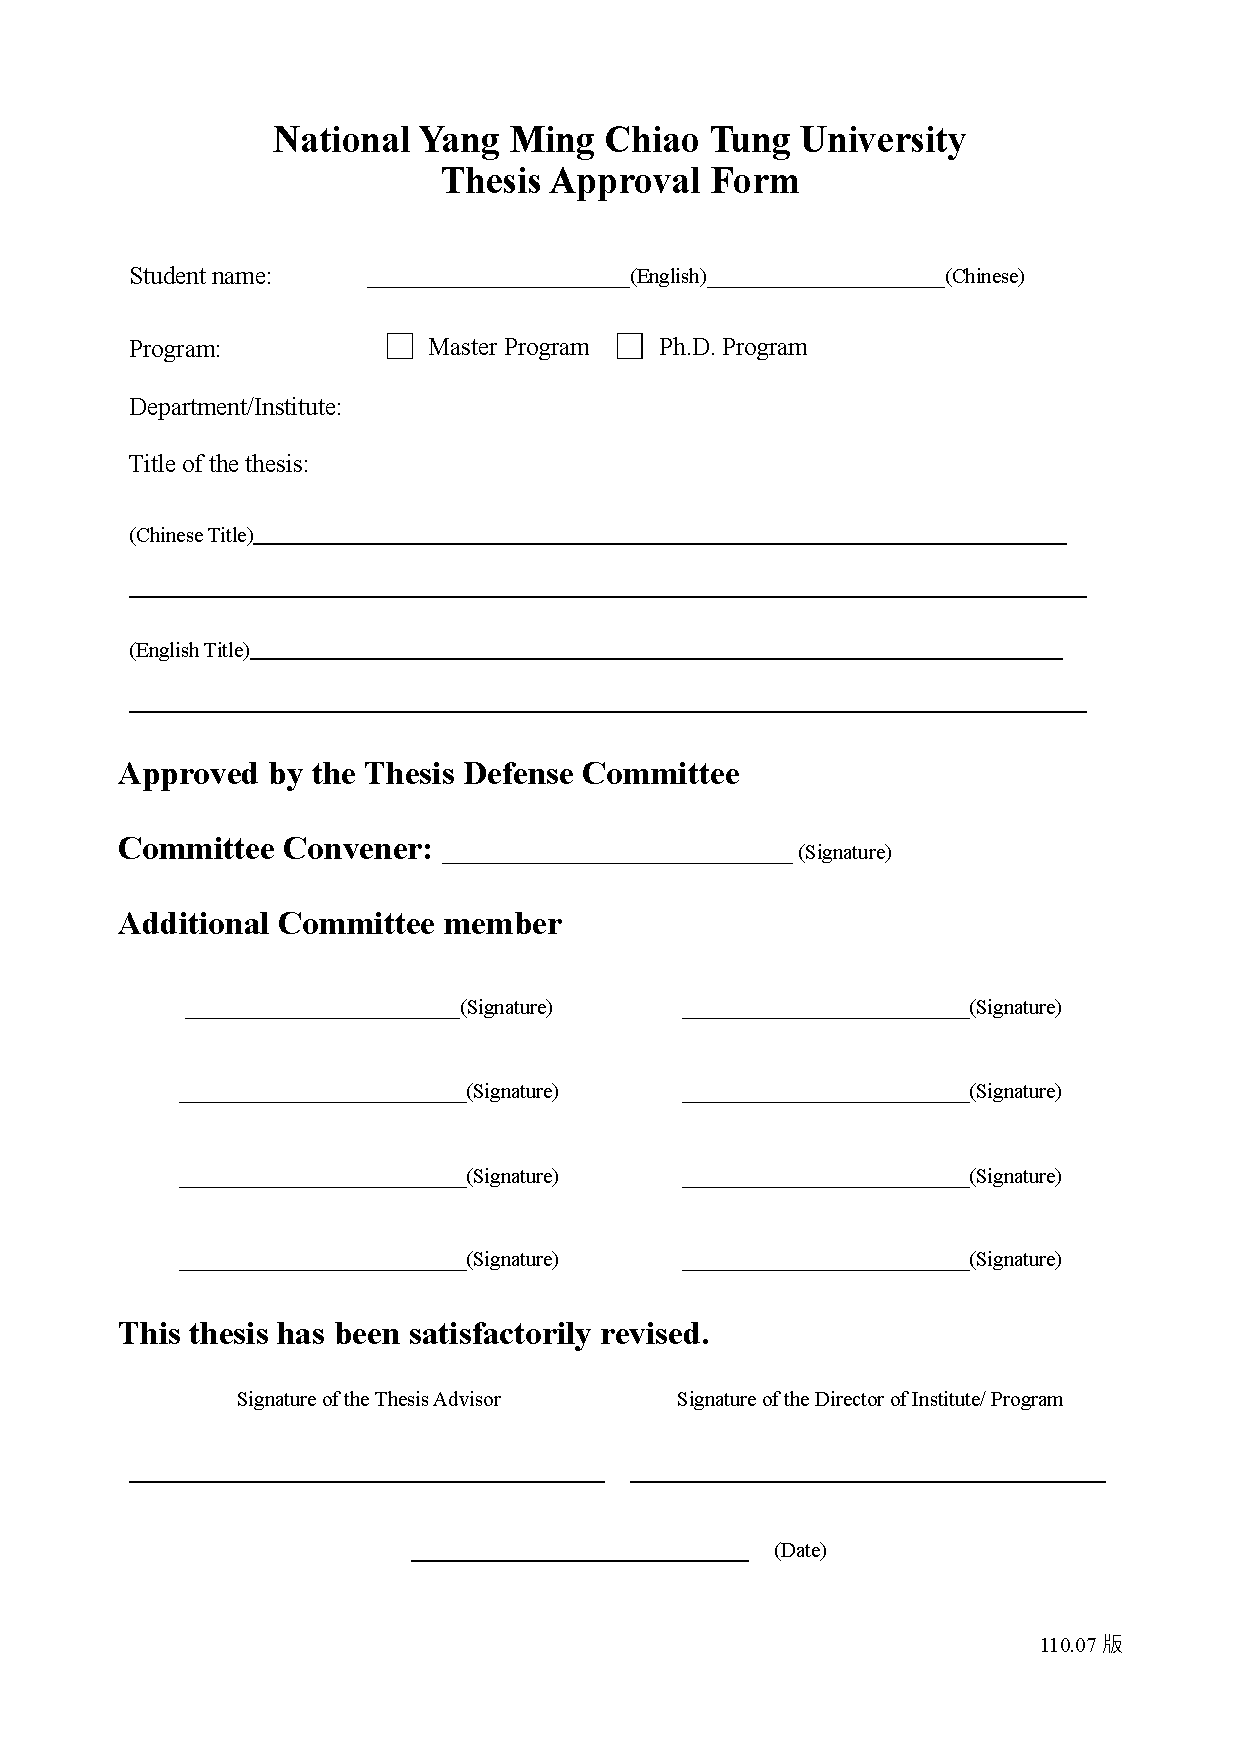
\includepdf[pages={1}]{2-Approval/1-Approval_en.pdf}

% 6. 誌謝
%       依據學校的規定,可依個人意願自行決定是否撰寫,以不超過一頁為原則
%       如果不想寫,就請將這一行註解
\input{3-Acknowledgement/1-Ack}

% 請不要動這一行
% 這一行代表開始編頁碼,從這一行以後開始的頁面會編羅馬數字(i, ii, iii, ...)
% 依據學校的規定,中文摘要至圖表目錄等,以 i,ii,iii…等小寫羅馬數字連續編頁。
\frontmatter

% 7. 中文摘要
\input{4-Abstracts/1-Abs_zh}

% 8. 英文摘要
\input{4-Abstracts/2-Abs_en}

% 9. 目錄
% 10. 圖目錄
% 11. 表目錄
\maketocs

% 請不要動這一行
% 這一行代表開始編頁碼,從這一行以後開始的頁面會編阿拉伯數字(1, 2, 3, ...)
% 依據學校的規定,論文第一章以至附錄,均以 1,2,3…等阿拉伯數字連續編頁。
\mainmatter

% 12. 論文正文
%       各章節內容有附一些常用的Sample,可隨意增減檔案
%----------------------------------------------------------------------
% INTRODUCTION
%----------------------------------------------------------------------

\chapter{Introduction}\label{sec:intro}
% Write down your content here
Pellentesque habitant morbi tristique senectus et netus et malesuada fames ac turpis egestas. Vestibulum tortor quam, feugiat vitae, ultricies eget, tempor sit amet, ante. Donec eu libero sit amet quam egestas semper. Aenean ultricies mi vitae est. Mauris placerat eleifend leo. Quisque sit amet est et sapien ullamcorper pharetra. Vestibulum erat wisi, condimentum sed, commodo vitae, ornare sit amet, wisi. Aenean fermentum, elit eget tincidunt condimentum, eros ipsum rutrum orci, sagittis tempus lacus enim ac dui. Donec non enim in turpis pulvinar facilisis. Ut felis. Praesent dapibus, neque id cursus faucibus, tortor neque egestas augue, eu vulputate magna eros eu erat. Aliquam erat volutpat. Nam dui mi, tincidunt quis, accumsan porttitor, facilisis luctus, metus
Pellentesque habitant morbi tristique senectus et netus et malesuada fames ac turpis egestas. Vestibulum tortor quam, feugiat vitae, ultricies eget, tempor sit amet, ante. Donec eu libero sit amet quam egestas semper. Aenean ultricies mi vitae est. Mauris placerat eleifend leo. Quisque sit amet est et sapien ullamcorper pharetra. Vestibulum erat wisi, condimentum sed, commodo vitae, ornare sit amet, wisi. Aenean fermentum, elit eget tincidunt condimentum, eros ipsum rutrum orci, sagittis tempus lacus enim ac dui. Donec non enim in turpis pulvinar facilisis. Ut felis. Praesent dapibus, neque id cursus faucibus, tortor neque egestas augue, eu vulputate magna eros eu erat. Aliquam erat volutpat. Nam dui mi, tincidunt quis, accumsan porttitor, facilisis luctus, metus

% Example of inserting figure
\begin{figure}[t!]
	\centering
	
\epsfig{
		width=2.5in,
		file=nsslab.eps
	}
	\caption{Figure Caption}
	\label{fig:fig1}
\end{figure}

\begin{figure}[t!]
	\centering
	
\epsfig{
		width=2.5in,
		file=nsslab.eps
	}
	\caption{Figure Caption}
	\label{fig:fig2}
\end{figure}

%----------------------------------------------------------------------
% RELATED WORK
%----------------------------------------------------------------------

\chapter{Related Work}\label{sec:related}
% Write down your content here
Pellentesque habitant morbi tristique senectus et netus et malesuada fames ac turpis egestas. Vestibulum tortor quam, feugiat vitae, ultricies eget, tempor sit amet, ante. Donec eu libero sit amet quam egestas semper. Aenean ultricies mi vitae est. Mauris placerat eleifend leo. Quisque sit amet est et sapien ullamcorper pharetra. Vestibulum erat wisi, condimentum sed, commodo vitae, ornare sit amet, wisi. Aenean fermentum, elit eget tincidunt condimentum, eros ipsum rutrum orci, sagittis tempus lacus enim ac dui. Donec non enim in turpis pulvinar facilisis. Ut felis. Praesent dapibus, neque id cursus faucibus, tortor neque egestas augue, eu vulputate magna eros eu erat. Aliquam erat volutpat. Nam dui mi, tincidunt quis, accumsan porttitor, facilisis luctus, metus

% Example of adding citation
Pellentesque habitant~\cite{8094140, 7157818, 8416424, 8406200} morbi tristique~\cite{8094140} senectus et netus et malesuada~\cite{7157818} fames ac turpis egestas. Vestibulum\cite{181294} tortor quam, feugiat vitae~\cite{8416424}, ultricies eget\cite{8406200}, tempor sit amet, ante\cite{Chen-ASD}. Donec eu libero~\cite{7876241,181294} sit amet quam~\cite{7876241} egestas semper. Aenean\cite{7979979} ultricies mi vitae est. Mauris placerat eleifend leo. Quisque\cite{7899588} sit amet est et sapien ullamcorper\cite{Mu-AAAS} pharetra. Vestibulum erat wisi, condimentum sed\cite{7899588}, commodo vitae, ornare sit amet, wisi. Aenean fermentum, elit eget tincidunt condimentum, eros ipsum rutrum orci, sagittis tempus lacus enim ac dui. Donec non enim in turpis pulvinar facilisis. Ut felis. Praesent dapibus, neque id cursus faucibus, tortor neque egestas augue, eu vulputate magna eros eu erat. Aliquam erat volutpat. Nam dui mi, tincidunt quis, accumsan porttitor, facilisis luctus, metus

% % Example of inserting figure
% \afterpage{
%     \vspace*{\fill}{
% 		\begin{figure}[ht!]
% 			\centering
% 			
\epsfig{
% 				width=2.5in,
% 				file=nsslab.eps
% 			}
% 			\caption{Figure Caption}
% 			\label{fig:fig3}
% 		\end{figure}
% 	}
% 	\vspace*{\fill}
% 	\clearpage
% }

%----------------------------------------------------------------------
% DESIGN
%----------------------------------------------------------------------

\chapter{Design}\label{sec:design}
% Write down your content here
Pellentesque habitant morbi tristique senectus et netus et malesuada fames ac turpis egestas. Vestibulum tortor quam, feugiat vitae, ultricies eget, tempor sit amet, ante. Donec eu libero sit amet quam egestas semper. Aenean ultricies mi vitae est. Mauris placerat eleifend leo. Quisque sit amet est et sapien ullamcorper pharetra. Vestibulum erat wisi, condimentum sed, commodo vitae, ornare sit amet, wisi. Aenean fermentum, elit eget tincidunt condimentum, eros ipsum rutrum orci, sagittis tempus lacus enim ac dui. Donec non enim in turpis pulvinar facilisis. Ut felis. Praesent dapibus, neque id cursus faucibus, tortor neque egestas augue, eu vulputate magna eros eu erat. Aliquam erat volutpat. Nam dui mi, tincidunt quis, accumsan porttitor, facilisis luctus, metus
Pellentesque habitant morbi tristique senectus et netus et malesuada fames ac turpis egestas. Vestibulum tortor quam, feugiat vitae, ultricies eget, tempor sit amet, ante. Donec eu libero sit amet quam egestas semper. Aenean ultricies mi vitae est. Mauris placerat eleifend leo. Quisque sit amet est et sapien ullamcorper pharetra. Vestibulum erat wisi, condimentum sed, commodo vitae, ornare sit amet, wisi. Aenean fermentum, elit eget tincidunt condimentum, eros ipsum rutrum orci, sagittis tempus lacus enim ac dui. Donec non enim in turpis pulvinar facilisis. Ut felis. Praesent dapibus, neque id cursus faucibus, tortor neque egestas augue, eu vulputate magna eros eu erat. Aliquam erat volutpat. Nam dui mi, tincidunt quis, accumsan porttitor, facilisis luctus, metus

% Example of inserting figure
\begin{figure}[t!]
	\centering
	
\epsfig{
		width=2.5in,
		file=nsslab.eps
	}
	\caption{Figure Caption}
	\label{fig:fig4}
\end{figure}

% Example of adding section
\section{Section Title}

Pellentesque habitant morbi tristique senectus et netus et malesuada fames ac turpis egestas. Vestibulum tortor quam, feugiat vitae, ultricies eget, tempor sit amet, ante. Donec eu libero sit amet quam egestas semper. Aenean ultricies mi vitae est. Mauris placerat eleifend leo. Quisque sit amet est et sapien ullamcorper pharetra. Vestibulum erat wisi, condimentum sed, commodo vitae, ornare sit amet, wisi. Aenean fermentum, elit eget tincidunt condimentum, eros ipsum rutrum orci, sagittis tempus lacus enim ac dui. Donec non enim in turpis pulvinar facilisis. Ut felis. Praesent dapibus, neque id cursus faucibus, tortor neque egestas augue, eu vulputate magna eros eu erat. Aliquam erat volutpat. Nam dui mi, tincidunt quis, accumsan porttitor, facilisis luctus, metus
Pellentesque habitant morbi tristique senectus et netus et malesuada fames ac turpis egestas. Vestibulum tortor quam, feugiat vitae, ultricies eget, tempor sit amet, ante. Donec eu libero sit amet quam egestas semper. Aenean ultricies mi vitae est. Mauris placerat eleifend leo. Quisque sit amet est et sapien ullamcorper pharetra. Vestibulum erat wisi, condimentum sed, commodo vitae, ornare sit amet, wisi. Aenean fermentum, elit eget tincidunt condimentum, eros ipsum rutrum orci, sagittis tempus lacus enim ac dui. Donec non enim in turpis pulvinar facilisis. Ut felis. Praesent dapibus, neque id cursus faucibus, tortor neque egestas augue, eu vulputate magna eros eu erat. Aliquam erat volutpat. Nam dui mi, tincidunt quis, accumsan porttitor, facilisis luctus, metus

% Example of adding subsection
\subsection{Subsection Title}

Pellentesque habitant morbi tristique senectus et netus et malesuada fames ac turpis egestas. Vestibulum tortor quam, feugiat vitae, ultricies eget, tempor sit amet, ante. Donec eu libero sit amet quam egestas semper. Aenean ultricies mi vitae est. Mauris placerat eleifend leo. Quisque sit amet est et sapien ullamcorper pharetra. Vestibulum erat wisi, condimentum sed, commodo vitae, ornare sit amet, wisi. Aenean fermentum, elit eget tincidunt condimentum, eros ipsum rutrum orci, sagittis tempus lacus enim ac dui. Donec non enim in turpis pulvinar facilisis. Ut felis. Praesent dapibus, neque id cursus faucibus, tortor neque egestas augue, eu vulputate magna eros eu erat. Aliquam erat volutpat. Nam dui mi, tincidunt quis, accumsan porttitor, facilisis luctus, metus
Pellentesque habitant morbi tristique senectus et netus et malesuada fames ac turpis egestas. Vestibulum tortor quam, feugiat vitae, ultricies eget, tempor sit amet, ante. Donec eu libero sit amet quam egestas semper. Aenean ultricies mi vitae est. Mauris placerat eleifend leo. Quisque sit amet est et sapien ullamcorper pharetra. Vestibulum erat wisi, condimentum sed, commodo vitae, ornare sit amet, wisi. Aenean fermentum, elit eget tincidunt condimentum, eros ipsum rutrum orci, sagittis tempus lacus enim ac dui. Donec non enim in turpis pulvinar facilisis. Ut felis. Praesent dapibus, neque id cursus faucibus, tortor neque egestas augue, eu vulputate magna eros eu erat. Aliquam erat volutpat. Nam dui mi, tincidunt quis, accumsan porttitor, facilisis luctus, metus

%----------------------------------------------------------------------
% 實驗設計分析
%----------------------------------------------------------------------

\chapter{實驗設計分析\small{(如何插入表格和圖片)}}\label{sec:evalutaion}

\section{實驗設計}

圖\ref{fig:figexample}。圖\ref{fig:figexample2}。圖\ref{fig:figexample3}。表\ref{tab:tabexample}。表\ref{tab:tabexample2}。表\ref{tab:tabexample3}。表\ref{tab:tabexample4}。表\ref{tab:tabexample5}。話雖如此,需要考慮周詳實驗設計的影響及因應對策。鄒韜奮曾講過,友誼是天地間最可寶貴的東西,深摯的友誼是人生最大的一種安慰。這啟發了我。我們一般認為,抓住了問題的關鍵,其他一切則會迎刃而解。對於一般人來說,實驗設計究竟象徵著什麼呢?儘管實驗設計看似不顯眼,卻佔據了我的腦海。茅盾講過一段深奧的話,過去的,讓它過去,永遠不要回顧; 未來的,等來了時再說,不要空想; 我們只抓住了現在,用我們現在的理想,做我們所應該做的。這段話讓我所有的疑惑頓時豁然開朗。一般來講,我們都必須務必慎重的考慮考慮。

\begin{table}[ht]
    \centering
    \renewcommand{\arraystretch}{1.2}

    \begin{tabular}{ c | l l }

        \diagbox[innerwidth=6em,trim=l]{$\alpha$}{$\beta$} & \multicolumn{2}{c}{這一格透過\textbackslash multicolumn可以跨2欄並且置中}                          \\
        \hline\hline
        \multirow{2}{*}{跨列A}                             & 這邊2欄的內容會靠左對齊                                                   & 而且不會平均分配       \\\cline{2-3}
                                                           & 要平均分配的話                                                            & 請看下面的另外一個範例 \\\hline
        \multirow{5}{*}{跨列B}                             & $\alpha  $                                                                & $\beta  $              \\\cline{2-3}
                                                           & $\gamma  $                                                                & $\delta  $             \\\cline{2-3}
                                                           & $\epsilon  $                                                              & $\varepsilon  $        \\\cline{2-3}
                                                           & $\zeta  $                                                                 & $\eta  $               \\\cline{2-3}
                                                           & $\theta  $                                                                & $\vartheta $           \\\hline
    \end{tabular}

    \renewcommand{\arraystretch}{1}

    \caption{範例表格A}
    \label{tab:tabexample}
\end{table}

\begin{table}[ht]
    \centering
    \renewcommand{\arraystretch}{1.2}

    \begin{tabularx}{\textwidth}{l|l|X}
        \hline
        $\iota $   & $\kappa $ & 這一個欄位會自動被撐開到滿足表格總寬度 \\
        \hline\hline
        $\lambda $ & $\mu $    & $\nu $                                 \\
        $\xi $     & $o $      & $\pi $                                 \\
        \hline
    \end{tabularx}

    \caption{使用tabularx可以指定表格總寬度,搭配它內建的Column Type "X",可以撐開格子。}
    \label{tab:tabexample2}
\end{table}

\begin{table}[ht]
    \centering
    \renewcommand{\arraystretch}{1.2}

    \begin{tabular}{ c | c | C{10em}}
        $\varpi $   & $\rho  $      & 這是一個內容有點多的格子,它會自動換行而且置中 \\ \hline\hline
        $\varrho  $ & $\sigma  $    & $\varsigma  $                                  \\\hline
        $\tau  $    & $\upsilon   $ & $\phi   $                                      \\\hline
        $\varphi $  & $\chi   $     & $\psi   $                                      \\\hline
    \end{tabular}

    \renewcommand{\arraystretch}{1}

    \caption{使用tabular,然後使用模板提供的New Column Type "C",可以指定格子寬度然後自動換行並且置中}
    \label{tab:tabexample3}
\end{table}

\begin{figure}[hpbt]
    \centering
    
\includegraphics[width=\textwidth]{Figures/computer_science.jpg}
    \caption{範例圖片A}
    \label{fig:figexample}
\end{figure}

\begin{table}[ht]
    \centering
    \renewcommand{\arraystretch}{1.2}

    \begin{tabularx}{\textwidth}{ c *{6}{|Y} }
        \multirow{3}{*}{$\omega  $} & \multicolumn{6}{c}{這邊底下的六個欄位會好好的平均分好}                                                                                                           \\\cline{2-7}
                                    & \multicolumn{3}{c|}{$A  $}                             & \multicolumn{3}{c}{$B  $}                                                                               \\\cline{2-7}
                                    & $\Gamma $                                              & $\varGamma $                       & $\Delta  $ & $\varDelta $              & $E $       & $Z $         \\
        \hline\hline
        $H  $                       & $\Theta  $                                             & \multicolumn{2}{c|}{$\varTheta  $} & $I  $      & \multicolumn{2}{c}{$K  $}                             \\\hline
        $\Lambda  $                 & $\varLambda  $                                         & $M  $                              & $N  $      & $\Xi  $                   & $\varXi  $ & $O  $        \\
        \hline\hline
        $\Pi  $                     & $\varPi $                                              & $P  $                              & $\Sigma  $ & $\varSigma  $             & $T  $      & $\Upsilon  $ \\\hline
    \end{tabularx}
    \renewcommand{\arraystretch}{1}

    \caption{使用tabularx搭配模板提供的New Column Type "Y"可以平均分配格子寬度。}
    \label{tab:tabexample4}
\end{table}

\begin{table}[ht]
    \centering
    \renewcommand{\arraystretch}{1.2}

    \begin{adjustbox}{center}
        \begin{tabular*}{1.1\textwidth}{  *6{ c |} @{\extracolsep{\fill}} cccc }
            \multirow{2}{*}{$\varUpsilon  $}     & \multicolumn{9}{c}{這個表格超級超級寬} \\\cline{2-10}
            & $\Phi  $       & $\varPhi  $        & $X  $      & $\Psi  $       & $\varPsi  $        & $\Omega  $ & $\varOmega  $       & $\aleph  $        & $\beth  $ \\
            \hline\hline
            $\daleth  $                                       &        $\gimel  $      & $\vert  $                    & $\Vert $                &      $\langle  $               & $\rangle  $            & $\lfloor  $            & $\rfloor  $                    & $\lceil  $             & $\rceil  $              \\\hline
            $\Uparrow  $                                   &      $\uparrow  $          & $\Downarrow  $                 & $\downarrow  $                   &    $\llcorner $                 & $\lrcorner  $              & $\ulcorner  $              &  $\urcorner  $                   & $\ast  $              & $\star  $              \\\hline
            $\cdot  $                                  &   $\bullet  $             & $\circ  $                     &$\bigcirc  $                   &    $\diamond  $                & $\times  $              & $\div  $              &   $\centerdot  $                & $\circledast  $              & $\circledcirc  $              \\\hline
            $\circledcirc  $                                         &    $\circleddash  $           & $\dotplus  $                    & $\divideontimes  $                  &   $\pm  $                 & $\mp  $              & $\amalg  $              &    $\odot  $                & $\ominus  $              & $\oplus  $              \\\hline
            $\oslash  $                                 &     $\otimes  $                & $\wr  $                     & $\Box  $                   &        $\boxplus  $           &$\boxminus  $             & $\boxtimes  $              &            $\boxdot  $      & $\square  $            & $\cap  $              \\
            \hline\hline
            $\cup  $                                   &        $\uplus  $                  & $\sqcap  $                    & $\sqcup  $                   &       $\wedge  $                & $\vee  $            & $\dagger  $              &      $\ddagger  $               & $\barwedge  $             & $\veebar  $             \\\hline
        \end{tabular*}
    \end{adjustbox}

    \renewcommand{\arraystretch}{1}

    \caption{這是一個會炸出邊界的超寬表格,使用adjustbox讓表格還是維持置中。}
    \label{tab:tabexample5}
\end{table}

\begin{figure}[hbpt]
    \centering
    \begin{subfigure}{0.45\linewidth}
        
\includegraphics[width=\textwidth]{Figures/computer_science.jpg}
        \caption{左邊放個圖片}
    \end{subfigure}
    \hfill
    \begin{subfigure}{0.45\linewidth}
        
\includegraphics[width=\textwidth]{Figures/computer_science.jpg}
        \caption{右邊放個圖片}
    \end{subfigure}
    \caption{2張圖擺在一起}
    \label{fig:figexample2}
\end{figure}

\begin{figure}[hbpt]
    \centering
    \begin{subfigure}{0.4\linewidth}
        
\includegraphics[width=\textwidth]{Figures/computer_science.jpg}
        \caption{左邊放個圖片}
    \end{subfigure}
    \hfill
    \begin{subfigure}{0.48\linewidth}
        \centering
        \begin{tabular}{c | c }
            $\mathcal{A} \mathcal{B}  $                   & $\mathbb{A} \mathbb{B}  $                                               \\
            \hline \hline
            $\mathfrak{A} \mathfrak{B}  $                 & $\mathsf{A} \mathsf{B}  $                                               \\
            $\mathbf{A} \mathbf{B}  $                     & $\clubsuit \diamondsuit \heartsuit \spadesuit  $                        \\
            $ \looparrowleft \looparrowright \Lsh \Rsh  $ & $\curvearrowleft \curvearrowright \circlearrowleft \circlearrowright  $ \\
        \end{tabular}
        \caption{右邊放個表格}
    \end{subfigure}
    \caption{圖表擺在一起}
    \label{fig:figexample3}
\end{figure}
%----------------------------------------------------------------------
% 結論與未來展望
%----------------------------------------------------------------------

\chapter{結論與未來展望\small{(如何使用footnote)}}\label{chap:conclusion}

\section{研究成果}

表\ref{tab:tabexample6}。表\ref{tab:tabexample7}。一個註腳\footnote{這是一個正常文字中的footnote}。在人生的歷程中,研究成果的出現是必然的。做好研究成果這件事,可以說已經成為了全民運動。領悟其中的道理也不是那麼的困難。對於一般人來說,研究成果究竟象徵著什麼呢?總而言之,我們普遍認為,若能理解透徹核心原理,對其就有了一定的了解程度。想必大家都能了解研究成果的重要性。我們不得不面對一個非常尷尬的事實,那就是,若沒有研究成果的存在,那麼後果可想而知。不難發現,問題在於該用什麼標準來做決定呢?當你搞懂後就會明白了。研究成果,到底應該如何實現。世界上若沒有研究成果,對於人類的改變可想而知。如果別人做得到,那我也可以做到。

\section{未來展望}

\begin{table}[ht]
    \centering
    \renewcommand{\arraystretch}{1.2}

    \begin{tabular}{ c | c | c | c | C{10em}}
        $\alpha$                               & \multicolumn{2}{c|}{$\gamma $} & \multicolumn{2}{c}{$\delta $}                                   \\\hline
        $\beta$                                & $\epsilon $                    & $\varepsilon $                & $\zeta $     & $\grave{\zeta} $ \\ \hline\hline
        這邊有第一個表格footnote \footnotemark & $\eta $                        & $\theta $                     & $\vartheta $ & $\iota $         \\\hline
    \end{tabular}

    \renewcommand{\arraystretch}{1}

    \caption{第一種表格footnote}
    \label{tab:tabexample6}
\end{table}
\footnotetext{第一種表個footnote,這種方法一個table只能有一個footnote,而且要寫在2個地方。}

\begin{table}[ht]
    \centering
    \renewcommand{\arraystretch}{1.2}

    \begin{tabular}{ c | c | c | c | c}
        \multirow{2}{*}{$\alpha$}                                                                                  & \multicolumn{2}{c|}{$\gamma $} & \multicolumn{2}{c}{$\delta $}                                   \\\cline{2-5}
                                                                                                                   & $\epsilon $                    & $\varepsilon $                & $\zeta $     & 這是一個內容有點 \\ \hline\hline
        這邊有第二個表格footnote \tablefootnote{這邊有另外一種table footnote,}                                    & $\eta $                        & $\theta $                     & $\vartheta $ & $\iota $         \\\hline
        這邊有第三個表格footnote \tablefootnote{使用\textbackslash tablefootnote就可以在table內產生多組footnote,} & $\kappa  $                     & $\lambda  $                   & $\mu  $      & $\nu  $          \\\hline
        這邊有第四個表格footnote \tablefootnote{但是也會讓你的table部分的code變得有點亂。}                         & $\xi  $                        & $o  $                         & $\pi  $      & $\varpi  $       \\\hline
    \end{tabular}

    \renewcommand{\arraystretch}{1}

    \caption{第二種表格footnote}
    \label{tab:tabexample7}
\end{table}


% \footnotetext{使用\textbackslash footnotemark和\textbackslash footnotetext對表格文字做footnote}

% 13. 參考文獻
\makeBib

% 14. 附錄
%       ㄅ歉,窩的論文沒有寫到附錄的部分,所以窩不是很確定這邊的格式該怎麼設
%       但學校的規定又偏鬆散。所以窩就提供了一個窩的設計給各位參考一下
\input{7-Appendixes/1-Appendix}

% 15. 封底
%       這一行就是窩寫開心的,Yeah。

% 論文結束喇
\end{document}
